\PassOptionsToPackage{dvipsnames}{xcolor}

\documentclass[12pt]{beamer}
\usetheme{default}
\usecolortheme{crane}

\usepackage[utf8x]{inputenc}
\usepackage[T1]{fontenc}
\usepackage[slovak]{babel}
\usepackage{ucs} % unicode

\usepackage{amsmath}
\usepackage{amsmath, amssymb}
\usepackage{hyperref, url}
\usepackage{graphicx}
\usepackage{array}
\usepackage{alltt}

%\setbeamersize{text margin left=1pt,text margin right=1pt}
\setbeamertemplate{footline}[frame number]
\beamertemplatenavigationsymbolsempty

% https://www.overleaf.com/learn/latex/Using_colours_in_LaTeX
\def\blue#1{\textcolor{Cerulean}{#1}}
\def\green#1{\textcolor{LimeGreen}{#1}}

% database-related stuff
\DeclareMathOperator{\join}{\bowtie}
\DeclareMathOperator{\antijoin}{\rhd}

\DeclareMathOperator{\lubi}{lubi}
\DeclareMathOperator{\capuje}{capuje}
\DeclareMathOperator{\navstivil}{navstivil}
\DeclareMathOperator{\vypil}{vypil}
\DeclareMathOperator{\answer}{answer}

\title{Transakcie}
\author{Ján Mazák}
\institute{FMFI UK Bratislava}
\date{}


\begin{document}

\frame{\titlepage}


\begin{frame}[fragile]{Transakcie}
\alert{Transakcie}, ktoré sa vykonajú celé, alebo vôbec nič z nich:
\begin{itemize}
\item riešia konzistenciu dát z hľadiska používateľov databázy;
\item riešia problém so zlyhaniami\\ (hardvér, výpadky siete či elektriny);
\item môže ich paralelne prebiehať mnoho,\\ navzájom o sebe nevedia.
\end{itemize}

\bigskip
Operácie v rámci transakcie:
\begin{itemize}
\item start (BEGIN TRANSACTION)
\item read (SELECT)
\item write (INSERT, UPDATE, DELETE)
\item \blue{COMMIT} (úspešné ukončenie) /\\\green{ROLLBACK} (abort, zrušenie)
\end{itemize}
\end{frame}


\begin{frame}[fragile]{Transakcie}
Príklad transakcie (PostgreSQL):
\begin{alltt}
    BEGIN;
    UPDATE accounts SET balance = balance - 100.00
        WHERE name = 'Alice';
    UPDATE accounts SET balance = balance + 100.00
        WHERE name = 'Bob';
    COMMIT;
\end{alltt}
\end{frame}


\begin{frame}[fragile]{Transakcie}
Príklad transakcie (Python):
\begin{alltt}
    command = 'INSERT INTO student VALUES (?, ?)'
    cursor = conn.cursor()
    cursor.execute(command, ('a', 'b'))
    cursor.execute(command, ('c', 'd'))
    conn.commit()
\end{alltt}
Príkaz pre začiatok transakcie sa odošle automaticky.
Databázové drivery zväčša umožňujú nastaviť tzv. \emph{autocommit} mód,
keď je každý vykonávaný príkaz transakciou sám osebe.
\end{frame}


\begin{frame}[fragile]{Transakcie}
Za prelínanie jednotlivých transakcií zodpovedá \blue{scheduler},
ktorý vytvára \alert{rozvrh} obsahujúci jednotlivé operácie (tiež \alert{história}).
Scheduler nevidí do budúcnosti a pre každú požiadavku jednotlivých transakcií
musí ihneď rozhodnúť, čo~s~ňou:
\begin{itemize}
\item vykonať hneď
\item počkať a skúsiť požiadavku zaradiť neskôr
\item abortnúť transakciu (napr. ak sa požiadavka nebude dať vykonať ani v budúcnosti, alebo ako prevenciu deadlocku)
\end{itemize}
\end{frame}


\begin{frame}[fragile]{Transakcie}
Dôvody abortu transakcie:
\begin{itemize}
\item explicitné želanie klienta
\item výpadok na strane klienta
\item výpadok na strane servera
\item strata spojenia medzi klientom a serverom
\item scheduler usúdi, že nie je možné v transakcii pokračovať\\
    (napr. by došlo k neriešiteľnému konfliktu s inou tx)
\end{itemize}
Klient musí počítať s tým, že dôjde k abortu jeho transakcie, aj keď všetky vykonal správne.
\end{frame}


\begin{frame}[fragile]{Požiadavky na transakcie --- \green{ACID}}
\begin{itemize}
\item \green{A}tomicity --- tx sa vykoná celá, alebo vôbec
\item \green{C}onsistency --- tx mení stav db z konzistentného na konzistentný (za toto zodpovedá klient)
\item \green{I}solation --- efekt paralelných transakcií je taký istý, ako keby boli vykonané postupne (v nejakom poradí)
\item \green{D}urability --- efekt tx musí po commite zotrvať aj pri výpadkoch systému
\end{itemize}
Reálne systémy niekedy čiastočne oslabia tieto garancie, aby zvýšili priepustnosť systému.
\end{frame}


\begin{frame}[fragile]{Rozvrhy}
\begin{minipage}{.4\pdfpagewidth}
\alert{Sériový}:\\
\\[5mm]
\begin{tabular}{c|c}
  $T_1$  & $T_2$  \\\hline\hline
  r(A)   &        \\\hline
  w(A)   &        \\\hline
  commit &        \\\hline
         & r(B)   \\\hline
         & w(C)   \\\hline
         & commit \\
\end{tabular}
\end{minipage}
\begin{minipage}{.4\pdfpagewidth}
Nie sériový,\\
ale \uv{ekvivalentný}:\\[5mm]
\begin{tabular}{c|c}
  $T_1$  & $T_2$  \\\hline\hline
  r(A)   &        \\\hline
         & r(B)   \\\hline
  w(A)   &        \\\hline
         & w(C)   \\\hline
         & commit \\\hline
  commit &        \\
\end{tabular}
\end{minipage}
\\[5mm]
Maximálna miera paralelizmu bez neželaných efektov: \alert{view-sériovateľnosť},
čiže \alert{view-ekvivalencia} nejakému sériovému rozvrhu.
\end{frame}


\begin{frame}[fragile]{Rozvrhy}
Dva rozvrhy $R$ a $S$ sú \alert{view-ekvivalentné}, ak:
\begin{itemize}
\item pozostávajú z tých istých transakcií;
\item ak $T_i$ je prvá tx v $R$, ktorá číta hodnotu objektu $X$, tak $T_i$ je prvá taká aj v $S$;
\item ak operácia $o_i$ z $T_i$ číta hodnotu zapísanú operáciou $o_j$ z $T_j$ v $R$, tak je to tak aj v $S$;
\item ak $T_i$ je posledná tx, ktorá zapisuje hodnotu objektu $X$ v $R$, tak $T_i$ je posledná taká aj v $S$;
\item tieto podmienky platia aj naopak (po výmene $R$ a $S$).
\end{itemize}
Čiže rozvrhy majú rovnaký efekt na výsledný stav databázy aj na výpočet jednotlivých transakcií.\\
\scriptsize{(Táto aj niektoré nasledujúce definície vynechávajú zopár technických detailov.)}
\end{frame}


\begin{frame}[fragile]{Rozvrhy}
V niektorých prípadoch môžu existovať rozvrhy, ktoré sú ekvivalentné sériovým,
ale nie sú view-sériovateľné --- vidno to však až z analýzy operácií iných ako READ a WRITE, a tie DBMS nevidí.

View-sériovateľnosť je nepraktická: je NP-ťažké rozhodnúť, či existuje view-ekvivalentný sériový rozvrh.
Preto sa prax zameriava na užšiu triedu rozvrhov (menej paralelizmu),
ktorá sa dobre generuje: konflikt-sériovateľné rozvrhy.
\end{frame}


\begin{frame}[fragile]{Rozvrhy}
Dve operácie na tom istom objekte z rôznych transakcií sú \alert{konfliktné} okrem prípadu read-read (čiže r-w, w-r, w-w).\\
Dva rozvrhy $R$ a $S$ sú \alert{konflikt-ekvivalentné}, ak:
\begin{itemize}
\item pozostávajú z tých istých transakcií;
\item poradie v rámci každej dvojice konfliktných operácií je v $R$ a $S$ rovnaké.
\end{itemize}
Rozvrh je \alert{konflikt-sériovateľný}, ak je konflikt-ekvivalentný nejakému sériovému rozvrhu.
\end{frame}


\begin{frame}[fragile]{Rozvrhy}
\begin{minipage}{.4\pdfpagewidth}
\begin{tabular}{c|c|c}
  $T_1$         & $T_2$         & $T_3$           \\\hline\hline
  \blue{w(A)}   &               &                 \\\hline
                & \green{r(B)}  &                 \\\hline
                & \blue{r(A)}   &                 \\\hline
                &               &  \alert{r(B)}   \\\hline
                &               &  \green{w(B)}   \\\hline
  \alert{w(B)}  &               &                 \\
\end{tabular}
\end{minipage}
\begin{minipage}{.4\pdfpagewidth}
Tento rozvrh \emph{nie je konflikt-sériovateľný}, lebo v akomkoľvek konflikt-ekvivalentom sériovom rozvrhu
by $T_1$ musela byť pred $T_2$ (modrá dvojica operácií), $T_2$ pred $T_3$ (zelená) a $T_3$ pred $T_1$ (červená).
(V tzv. precedenčnom grafe, ktorý možno zostaviť z hrán zodpovedajúcich konfliktným operáciám, sa vyskytuje cyklus.)
\end{minipage}
\\[5mm]
\end{frame}


\begin{frame}[fragile]{Rozvrhy}
V niektorých prípadoch možno z požiadaviek na sériovateľnosť zľaviť.
\begin{itemize}
\item read-only transakcie
\item zisťovanie databázových štatistík pre účely optimalizácie dotazov (stačí nám aproximácia výsledkov)
\item distribuované databázy (zabezpečiť sériovateľnosť môže byť pridrahé)
\end{itemize}
Vo všeobecnosti si volíme kompromis medzi výkonom a mierou izolácie (a konzistencie).
\end{frame}


\begin{frame}[fragile]{Obnoviteľnosť}
Aby bolo možné zabezpečiť požiadavku na trvalé uchovanie dát (durability), musia byť rozvrhy odolné voči výpadkom DBMS.

Najjednoduchším riešením je pred každou operáciou do logu (žurnálu) zapísať,
že ju ideme vykonať.
Jednotlivé operácie môžu byť pomerne náročné (napr. po pridaní záznamu treba upraviť index či spustiť trigger)
a nedajú sa vykonávať atomicky, ale samotný zápis do logu áno.
Log zároveň rieši problémy s rôznymi vyrovnávacími pamäťami (cache manažér môže pozdržať zápis bloku na disk apod.).
\end{frame}


\begin{frame}[fragile]{Obnoviteľnosť}
V prípade pádu systému sa len pozrieme do logu,
odstránime efekt transakcií, ktoré treba abortnúť (UNDO), a vykonáme operácie commitnutých transakcií nanovo (REDO).
\\[3mm]

Správa logu využíva prostriedky operačného systému a nemusí byť úplne spoľahlivá: príkladom je sekcia
\uv{How To Corrupt Your Database Files} v dokumentácii SQLite
(\href{https://www.sqlite.org/lockingv3.html#rollback}{link}).
\end{frame}


\begin{frame}[fragile]{Obnoviteľnosť}
Príklad rozvrhu, ktorý \alert{nie je obnoviteľný}:\\[5mm]
\begin{minipage}{.4\pdfpagewidth}
\begin{tabular}{c|c}
  $T_1$         & $T_2$        \\\hline\hline
  \blue{w(A)}   &              \\\hline
                & \blue{r(A)}  \\\hline
                & w(B)         \\\hline
                & commit       \\\hline
  commit        &              \\
\end{tabular}
\end{minipage}
\begin{minipage}{.4\pdfpagewidth}
Dvojica modrých operácií predstavuje \alert{dirty read}:
$T_2$ číta hodnotu, ktorá ešte nie je commitnutá, a ak by došlo k výpadku po commite $T_2$, ale pred commitom $T_1$,
hodnoty vypočítané $T_2$ budú vychádzať z falošnej hodnoty objektu A (ktorá nikdy nebola zapísaná do db).
\end{minipage}
\\[12mm]
\end{frame}


\begin{frame}[fragile]{Obnoviteľnosť}
Uvedený rozvrh sa dá napraviť výmenou poradia commitov.\\[5mm]
\begin{minipage}{.4\pdfpagewidth}
\begin{tabular}{c|c}
  $T_1$         & $T_2$        \\\hline\hline
  \blue{w(A)}   &              \\\hline
                & \blue{r(A)}  \\\hline
                & w(B)         \\\hline
  commit        &              \\\hline
                & commit       \\
\end{tabular}
\end{minipage}
\begin{minipage}{.4\pdfpagewidth}
Je tu však ďalší problém: abort $T_1$ (miesto commitu) povedie k vynútenému abortu $T_2$ (\emph{cascading abort}).
Takto sa abort môže šíriť do ďalších transakcií a musíme zahodiť všetku prácu, čo vykonali.
\end{minipage}
\\[5mm]
Riešenie: generovať rozvrhy, ktoré vôbec neobsahujú \emph{dirty read} (trieda ACA --- avoids cascading aborts),
príp. ani \emph{dirty write} (\alert{striktné} rozvrhy).
\end{frame}


\begin{frame}[fragile]{Rozvrhy}
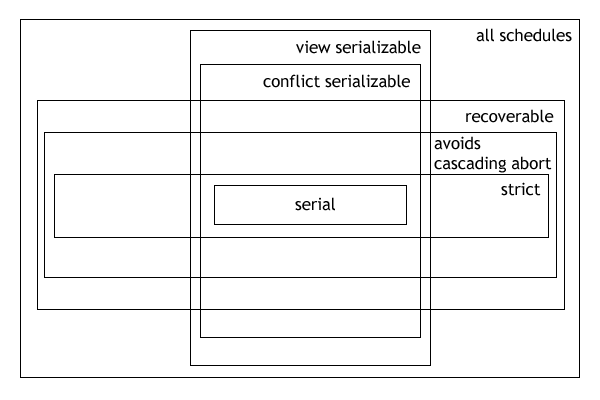
\includegraphics[scale=2]{rozvrhy.png}

Všeobecne zamerané DBMS využívajú najmä konflikt-sériovateľné striktné rozvrhy.
\end{frame}

\begin{frame}[fragile]{Rozvrhy}
Metódy na generovanie vyhovujúcich rozvrhov:
\begin{itemize}
\item dvojfázové zamykanie
\item časové pečiatky
\item validácia
\item multi-version concurrency control (MVCC)
\item \dots
\end{itemize}
\end{frame}

\begin{frame}[fragile]{Zámky}
Základnou technikou na generovanie konflikt-sériovateľných rozvrhov je použitie zámkov.
\alert{Zámky} môžu mať rôznu granularitu (záznam, celá tabuľka apod.). Typy zámkov:
\begin{itemize}
\item exkluzívne (write lock)
\item zdieľané, len na čítanie (read lock)
\item upgrade lock atď.
\end{itemize}
Pred vykonaním operácie musí transakcia dostať zámok, ktorý jej umožní túto operáciu vykonať.
V minimalistickej verzii sa využijú len exkluzívne zámky, čiže prvá tx dostane prístup k objektu
a ostatné musia čakať (alebo budú abortnuté). Využitie zdieľaných zámkov výrazne urýchli prácu systému,
v ktorom sa veľa číta a menej zapisuje.
\end{frame}


\begin{frame}[fragile]{Dvojfázové zamykanie}
Princíp dvojfázového zamykania (2PL) --- v prvej fáze transakcia zámky získava,
v druhej už len uvoľňuje. Pre dvojicu konfliktných operácií dochádza aj ku konfliktu zámkov
(nemôžu byť pridelené súčasne pre obe operácie).\\[2mm]

\blue{2PL generuje len konflikt-sériovateľné rozvrhy.}\\[2mm]

(Predpokladajme opak. Potom musí v precedenčnom grafe existovať cyklus,
povedzme $T_1 \rightarrow T_2 \rightarrow \dots \rightarrow T_1$.
Ak $T_i$ predchádza $T_j$, tak v príslušnej dvojici konfliktných operácií $T_j$ dostane zámok až po tom,
čo ho $T_i$ uvoľnila.
Potom však $T_1$ musí získať zámok až potom, čo ho uvoľnila, a to je spor s definíciou 2PL.)
\end{frame}


\begin{frame}[fragile]{Striktné dvojfázové zamykanie}
Ak pridáme k 2PL požiadavku na uvoľnovanie zámkov len pri commite (Strict 2PL), zníži to mieru paralelizmu
(niektoré rozvrhy generované 2PL už nebudú vyhovovať), ale zabezpečí generovanie striktných rozvrhov.\\[2mm]

Po zápise hodnoty do zdieľaného objektu bude transakcia držať exkluzívny zámok na tento objekt až do svojho commitu
a medzitým žiadna tx nemôže na tento objekt získať zámok, čiže žiaden dirty read (ani write) nemôže nastať.\\[2mm]

\scriptsize{Poznámka: Zdieľané zámky by bolo možné uvoľňovať aj skôr ako pri commite,
ale v~praxi to nevedie k pozorovateľnému zrýchleniu a pridáva overhead.
Uvoľňovanie zámkov pri commite je veľmi ľahké implementovať v podobe online algoritmu:
nepotrebujeme vidieť \uv{budúce} operácie tx, aby sme vedeli, kedy uvoľňovať zámky.}
\end{frame}

\begin{frame}[fragile]{Dvojfázové zamykanie}
Rozvrh vytvorený 2PL môže viesť k \alert{deadlocku}:
vzniku cyklu transakcií, z ktorých každá čaká, kým predošlá uvoľní nejaký zámok, ktorý ona potrebuje.

Deadlocky možno riešiť v momente, keď nastanú (udržiavame graf čakajúcich transakcií a detekujeme v ňom cykly),
alebo ich vzniku predchádzať niektorou zo známych metód
(idea je zachovať staršie transakcie, ktoré už nejakú prácu vykonali):
\begin{itemize}
\item \blue{wait-die}\\ (ak novšia tx žiada zámok od staršej, abortneme novšiu);
\item \blue{wound-wait}\\ (ak staršia tx žiada zámok od novšej, spôsobí jej abort).
\end{itemize}
\end{frame}


\begin{frame}[fragile]{Izolácia transakcií podľa SQL štandardu}
Štandard SQL vychádza z neželaných javov pri paralelnom behu transakcií.
\begin{itemize}
\item \alert{dirty read}
\item \alert{nonrepeatable read} (tx prečíta 2x po sebe ten istý záznam, ale dostane rôzne výsledky)
\item \alert{phantom read} (tx si vyžiada 2x záznamy určené tou istou podmienkou, ale dostane rôzne výsledky)
\item \alert{serialization anomaly} (výsledok rozvrhu niekoľkých tx nezodpovedá žiadnemu ich sériovému rozvrhu)
\end{itemize}
\end{frame}

\begin{frame}[fragile]{Izolácia transakcií podľa SQL štandardu}
Štandardné úrovne izolácie a ich implementácia v PostgreSQL:
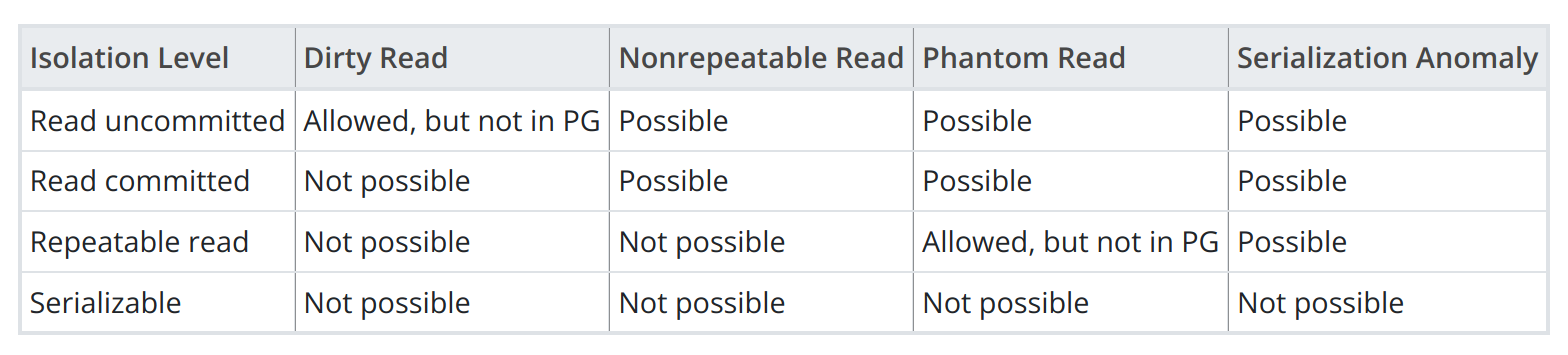
\includegraphics[scale=.2]{isolationLevels.png}\\[2mm]

Default by mal byť podľa štandardu \verb|SERIALIZABLE|, ale pre väčšinu DBMS to tak nie je.
Úroveň izolácie si vie transakcia zvoliť na začiatku, napr.
\begin{alltt}
  BEGIN TRANSACTION ISOLATION LEVEL REPEATABLE READ;
\end{alltt}

Existujú aj možnosti nad rámec štandardu, napr. \verb|READ ONLY| transakcie.

\end{frame}

\begin{frame}[fragile]{Izolácia transakcií podľa SQL štandardu}
PostgreSQL využíva MVCC (výhodou oproti zamykaniu je, že čítanie a zapisovanie sa navzájom neblokujú).
Pred verziou 9.1 (cca 2011) v PostgreSQL chýbala implementácia skutočného SERIALIZABLE levelu
(lebo pre MVCC to vymysleli až v 2008).\\[5mm]

Paralelné spracovanie môže viesť k vzniku chýb, za ktoré samotná tx nemôže a nevie ich ovplyvniť, napr.
{\scriptsize
\begin{alltt}
    ERROR:  could not serialize access due to concurrent update
\end{alltt}
}

{\small
Nepovinné čítanie o nesúlade teórie a praxe izolácie transakcií:\\
A Critique of ANSI SQL Isolation Levels (2007) (\href{https://arxiv.org/abs/cs/0701157}{link})
}
\end{frame}






\begin{frame}{Literatúra}
\begin{itemize}
\item {\scriptsize\url{https://cs186berkeley.net/notes/note11/}}
\item {\scriptsize\url{https://cs186berkeley.net/notes/note12/}}
\item {\scriptsize\url{https://www.db-book.com/slides-dir/PDF-dir/ch17.pdf}}
\item {\scriptsize\url{https://www.db-book.com/slides-dir/PDF-dir/ch18.pdf}}
\item {\scriptsize\url{https://www.db-book.com/slides-dir/PDF-dir/ch19.pdf}}
\item {\scriptsize\url{https://en.wikipedia.org/wiki/Database_transaction_scheduling}}
\item {\scriptsize\href{https://www.postgresql.org/docs/current/mvcc.html}{Transaction isolation in PostgreSQL}}
\item {\scriptsize\href{https://www.sqlite.org/isolation.html}{Transaction isolation in SQLite}}
\end{itemize}
\end{frame}

\end{document}
